\graphicspath{{mechanism/}}

\chapter{Teaching the Mechanism of the Greenhouse Effect}
\label{chap:mechanism}


Notes - this is the most straightforward approach, and in line with
``classical'' approaches to education (to be contrasted with NDI).

\section{Actual Abstract (delete heading before finishing)}

As described above, American's are about split over acceptance of anthropogenic
climate change. Informally, Michael Ranney, then other members of our group
started questioning whether people were able to mechanistically explain how
greenhouse gases cause an increase in global mean temperature. Almost no one
could provide such an explanation. In this experiment, we sought to formally ask
whether this lack of understanding is indeed as pervasive as it seemed to be.
Critically, we suspected that a mechanistic comprehension of global climate
change might increase individual's acceptance of the reality of anthropogenic
climate change, and ultimately help pave the way towards addressing this
critical problem.

In this exploratory study, we also probed RTMD-relevant attitudes both
before and after participant's receive our explanation. In addition, we asked
participants if they experienced any surprise at our explanation. In this way,
we were able to see in what ways RTMD and multi-system learning might be
explored in future experiments.

% Ryan thinks this is unconvincing, game-show like. Could make a parallel with
% Jame's psychophysical experiments, where people could clearly know that an
% apple is read, but they need to be trained to report the basic visual
% properties of what they see preferentially over reporting "basic level"
% phenomena. The "basic pieces" of our mechanism do indeed seem new to most, but
% we have yet to formally test that part.

At present, our group has obtained responses both for 103 Berkeley
undergraduates, and 49 from two classes at UT, Brownsville. For now, we have
only prepared results from the Berkeley undergrads, and the work has been
presented in the format of a talk along with a brief mention in
\citeauthor{ranney_why_inpress}.  

\section{Classroom interventions at UC and UT}

The general form of the intervention was quite simple. Participants were split
into two groups. Both groups read an educational blurb regarding the mechanism
of greenhouse gasses, and indicated any surprise they may have experienced.
After this, participants completed a knowledge and attitude test. For one group,
they completed an identical knowledge and attitude test prior to the educational
blurb - making a kind of test ``sandwich'' filled with nutritious explanations
of climate change. Continuing this metaphor, the other group, with it's single
post-test is more like an ``open-faced'' (sandwich) group.\footnote{In this
    metaphor, temporal order extends from top to bottom, as with an object
    falling with gravity.}

Of central interest was verifying that almost no-one actually knows the
mechanism for climate change. And, while analyses are still in progress, we:

\begin{enumerate}
    \item Assessed the effectiveness of a mechanistic explanation in eliciting
        attitude shifts.
    \item Assessed RTMD relationships.
    \item Evaluated the predictiveness of surprise in learning and attitude shifts.
    \item Observed the effects of a pre-test on participants' surprise ratings.
\end{enumerate}

In subsequent analyses, we will do a more careful analysis of the actual
learning that occurred (this has only recently been coded from written responses).


\subsection{Experimental Methods}

This experiment was a fairly thick observation of individuals' beliefs,
attitudes and knowledge. We sought to understand how a relatively brief 400-word
mechanistic explanation might affect these measures, as well as how this might
be modulated by prior commitment to one's own explanations.

\subsubsection{Participants}

As mentioned above, at present, we have collected data from 103 Berkeley
undergraduates, and 49 from two classes at the University of Texas,
Brownsville.

\subsubsection{Materials}

Participants received:

\begin{enumerate}
    \item 400-word description of the mechanism 
        by which greenhouse gases effect global mean temperature increase (in our
        piloting, this description could be read in about 2 minutes)
    \item RTMD attitude survey
    \item 3 short essay questions testing participant knowledge of the above mechanism
    \item 2 knowledge fill-in-the-blank items on light entering / exiting troposphere
    \item Demographic survey
\end{enumerate}

\subsubsection{Procedure}

Participants were run simultaneously for each of the two classes. Instructions
were administered by the course instructor, and students received one of two
packets---placing them into one of the two groups described above. After
completing the consent form on the front of the packet, individuals proceeded to
read and answer questions. The entire experiment was completed in approximately
25 minutes.

\subsubsection{Analysis}

Handwritten responses were coded and placed into a spreadsheet. Given the rich
nature of these data, many analyses were employed. In brief, when appropriate,
straight t-tests were used, and in evaluating the relationships between RTMD
constructs, confirmatory factor analysis was employed.

\subsection{Results}

First off, individuals definitely did not have a clear mechanistic understanding
of how greenhouse gases contribute to global warming. Prior to instruction,
\emph{no} participants indicated anything about different kinds of radiation, or
atmospheric retention time for the sun's energy. Afterwards, though,
participants were often able to at least recall some basic details. For example,
40/103 described something about different kinds of radiation and 37/103
explained that energy was retained in the atmosphere. A more careful analysis
will be done shortly using the recently completed coding of textual items.

Participants shifted on average 14\% closer to ``extreme'' agreement with climate
change items. Combining groups using an imputation approach, this was
significant ($t(72)=2.28, p=.01$). There was no difference between groups on the post-test. In fact, the open-faced
group actually had a slightly greater global warming acceptance
attitude as compared to the sandwich group on average. 

Participants reported greater surprise when they were required to commit to
their own description before instruction ($t(42.1)=1.7, p=.05$). These surprise
ratings were increased from a mean of 2.3 to 3.0 on a 9-point scale. It
surprises us that their ratings are so low in general! Overall, a broad range of
surprise ratings, spanning the scale was observed. Ratings from 7 to 9 were only
observed in the Sandwich condition.

\begin{figure}[h]
    \centering
    \subfloat{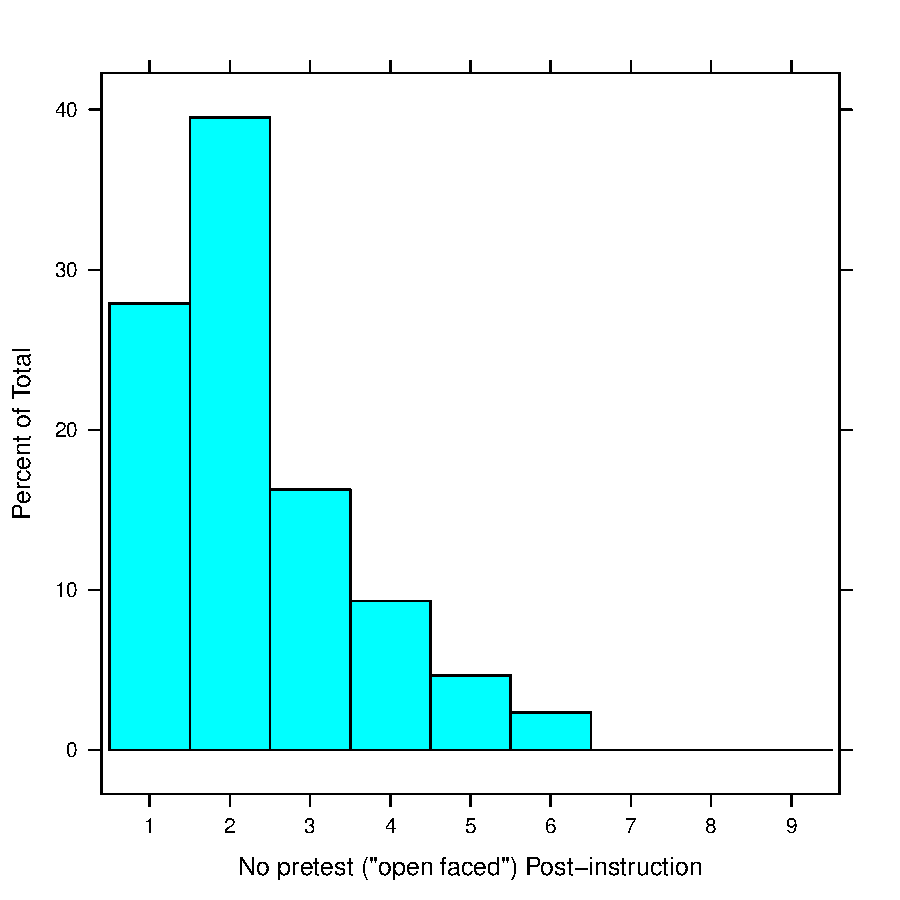
\includegraphics[width=0.5\textwidth]{hypotheses-surprisedistributions1.pdf}}
    \subfloat{\includegraphics[width=0.5\textwidth]{hypotheses-surprisedistributions2.pdf}}
    \caption{Distributions of surprise ratings for the sandwich and open-faced
        groups, note the slight increase in ``1'' ratings (which may indicate resistance
        to the intervention) co-occurs with an increase (from none) in ratings 7-9 in
        the sandwich group.}
    % For final, re-do these graphs so they have the same y-scales
\end{figure}

Note, I suspect it is unlikely that individuals experienced the same kind of
``visceral'' surprise from the blurb that can be obtained by, for example,
statistics we've used regarding things like abortion and the death penalty. And,
while it may be due to a limitation of imagination, I have difficulty imagining
an evolution item that would elicit this kind of surprise.

In addition, we replicated the relationships predicted by the RTMD theory in
another population. Confirmatory factor analysis yielded quite similar results
to simple correlation tables between the means of attitude-relevant items. In
particular, all proximal relationships held in this population (those
represented by lines in Figure~\ref{fig:rtmd}) and in each survey, either 12 or
13 out of 15 total relationships were in the direction predicted by RTMD. Less
formally, it appears that the correlations between evolution and climate change
increased after our intervention---perhaps indicating a shift in which
participants viewed climate change as part of ``real science.'' Similar
increases in anti-correlation with nationalism were observed. However, we have
not yet established appropriate statistical machinery to test the significance
of these effects.

\subsection{Discussion}

In general, we have established quite clearly that individuals are largely
ignorant of the mechanism via which greenhouse gases cause global warming,
suggesting that this is a reasonable object of study! More specifically, even
this (relatively dry) 400-word blurb was able to effect shifts in attitudes and
elicit non-trivial surprise ratings from individuals. It remains to see how
attitude shifts and learning are related, but the results as they are seem
sufficient basis for proceeding on an educational research program including
mechanism!


% This should be placed in the correct location above

\begin{figure}
    \begin{center}
        \includegraphics{causal2.pdf}
    \end{center}
    \caption{A graphical model representing the relationship between forms of
        psychological processing of factual information observed in
        chapter~\ref{chap:mechanism}. Here, the relationship between pre-existing
        information and surprise was the result of an experimental manipulation and
        is assumed to be causal.}
    \label{fig:causal-mechanism}
\end{figure}

\section{A web-based intervention with UC Undergrads}

Given the replicated demonstrations of significant attitude changes described
above, we proceeded to assess whether the mechanism-explanation effects we had
obtained were durable rather than transient. This study extended prior work by
delaying the post-test several days. We also wondered whether an ``experimental
demand'' from the classroom setting might have driven our prior results, so we
provided the intervention on-line; that is, we assessed whether our materials
would elicit significant attitude change even though students participated via
their own computers, without experimenter observation. Thus we concurrently
explored the longevity (via delay) and format (on-line) aspects of our
phenomenon. We also extended our prompts to incorporate more demographic and
introspection queries.

\subsection{Methods}

The survey and instructional materials were those reported in Ranney et
al. (2012a \& 2012b; the latter includes the full 400-word text of our
intervention). The primary difference was that administration was conducted
entirely online, via the Qualtrics Inc. (Provo, UT) system. Eight items were
added to pre- and post-test attitude surveys to add reliability to the related
RTMD metrics (specifically, national and religious affinities; these metrics
will be reported elsewhere). Five further questions were introduced immediately
following the instructional material to elicit introspection (about
embarrassment, disagreement, etc.).  Undergraduates (N=80) were recruited via
the Research Participation Program (RPP), administered by the University of
California, Berkeley (UCB) psychology department. Such recruitment allowed us to
administer a pre-test to about half of the students (38) between 8 and 26 days
($\mu=18.5$ days) before any of the 80 participated in the study, which may have
allayed test-retest effects (although Ranney et al., 2012a, found little
evidence for them). Thus, as with Ranney et al. (2012a), some participants
received the full survey testing ``sandwich'' while others had no pre-test. A
delayed post-test was given to all participants between 1 and 8 days later
($\mu=4$ days). This range was used to assess the timecourse of retention in
planning subsequent studies, We lack the power to test forgetting over time here
(though numerically, did not observe any!).

\subsection{Results and Discussion} 

Split this up! Note results have changed a bit for Knowledge (both kinds) using
regression and glht. Should also do something more definitive with the GW
attitude data (though this was unchanged for the CogSci paper).

In general and as anticipated, we replicated Ranney et
al.’s (2012a) results and extended them by finding that shifts were retained
over the mean (four-day) delay. 
% Include more verbiage here explaining lme4, Anova and glht
Scored knowledge was comparable to previously
tested UC students, rising from 3.8 on pre-test to 6.5 post-test and 6.3 on
followup (gains from pre-test were significant at $p<0.0001$ for both subsequent
scores). GW belief ratings (with higher ratings being
more in concert with science’s consensus) increased from a 6.20 pre-test mean to
a 6.54 post-test mean ($t(79)=2.5, p=0.006$; a healthy improvement on our 1-9
Likert scales!). Some of this improvement
diminished over the following days, but most was retained: the mean score on the
delayed post-test was 6.44 (t(79)=1.7, p=0.05). Self-rated knowledge means
increased markedly from pre- to post-test (4.5 to 5.6 on a 9-point scale,
t(79)=8.5, p<0.001). Retention of this increase, gratifyingly, was also noted on
the delayed post-test (5.2, t(79)=6.2, p<0.001). (The immediate increase in
self-rated knowledge, in fact, replicates results from the ``sandwich''
interventions in Ranney et al., 2012a, though those results were not reported.)

\subsubsection{Micro-analysis of GW ratings}

Table~\ref{table:uc-online-gw-means} reports the mean rating across participants
for agreement with individual items (For the full text of these items, see
Appendix~\ref{app:survey-items}). The largest gains were found in agreeing with
``Human activities are largely responsible for the climate changes\ldots'' (a
0.25 gain) and certainty that global warming is occurring (a 0.19 gain).  In
general, gains were fairly consistent across all GW measures, ranging only
down to 0.11 at the lowest (the über-greenie “humans are severely abusing the
environment”). Interestingly importance of lifestyle changed the most
(0.27, though this was not included in the tested average gw variable).
Expectation of engagement, dishearteningly, clocks in at a 0.05 \emph{drop}! 
% Enter motivational interventions like Oroeco?

% latex table generated in R 2.15.1 by xtable 1.7-1 package
% Thu May  9 12:43:59 2013
\begin{table}[h]
\caption{Mean GW ratings, online with UC undergrads} 
\label{table:uc-online-gw-means}
\centering
\begin{tabular}{rccc}
  \toprule
 & pre & pst & fol \\ 
  \midrule
  gw1\_2 & 6.61 & 6.86 & 6.36 \\ 
  gw2\_1 & 5.19 & 5.31 & 5.25 \\ 
  gw2\_2 & 6.61 & 6.81 & 6.67 \\ 
  gw2\_3 & 5.81 & 5.97 & 5.97 \\ 
  gw2\_4 & 6.78 & 6.86 & 6.67 \\ 
  engage & 5.91 & 5.86 & 6.11 \\ 
  lifesty & 4.83 & 5.11 & 4.94 \\ 
  \bottomrule
\end{tabular}
\end{table}



\subsubsection{Correlations}

Scored knowledge and self-rated knowledge are significantly correlated pre-test,
so participants have decent meta-cognition here.
% TODO: insert statistics from Retention notebook in RPP_Su2012

\subsection{Interim conclusion}

In sum, this study extends the finding that well-considered information, even
received online, increases anthropogenic global warming acceptance and
behaviorally relevant attitudes; the conceptual changes that result from reading
even 400 words have notable longevity. These effects have been replicated with
members of the general public as well (unpublished data). Computer-based
interventions often scale well, enhance reliability, and prove cost-effective;
given our results, we recommend the online distribution of mechanistic
explanations, especially about climate change.  

% Currently, this is just significant results for the UC CogSci class (2010?)
% from “general improvements”
\extrarowsep 5pt
% copy pasted from mechanism/uc-classroom-summary.csv
% below can use siunitx, and \num with \sisetup{round-precision=2,round-mode=figures,scientific-notation=true}
% I like table-parse-only. This doesn't work somehow: [table-number-alignment = center]
\begin{longtabu}{X[2.5]S[table-parse-only]X[l]}

% Final \\ necessary to compile!
\caption{Summary of results for college classroom interventions \label{table:summary-classroom}}\\
\toprule
Result & {$p$-value} & Statistic \\ \midrule
\endfirsthead

% The empty option prevents a TOC entry from being generated
\caption[]{College classroom interventions, continued}\\
\toprule
Result & {$p$-value} & Statistic \\ \midrule
\endhead

\bottomrule
\endfoot

People don't tend to mention the mechanism in pre-test (11/42), but they do in
post-test (S post is 26/30, N is 39/43 - stat computed for S group pre- vs.
post-, which has a lesser prevalence of mech than N) & 3.20E-07 &
Fisher's exact "two-sided" \\
Misconceptions are common in the pretest but not the post test, total 0.38 pre-
to 0.10/0.12 (S/N) post-test. Ozone .19 to .03/.02 (S/N),  wrong GHG  .24 to
0.07/0.09 (S/N). (test on total misconceptions, S pre- to post-test) & 0.01
& Fisher's exact "two-sided" \\
Participants don't mention energy leaving the earth until prompted.
Specifically, of the four codes that deal with this topic, only 6 mention
something about "trapped heat" in the pre-test on the first (i.e., the only
unscaffolded) question. & 0.0002 & Fisher's exact "two-sided" \\
Use of infrared is greater post-test than pre-test. Goes from 0 to 16 / 22 in S
/ N groups. & 3.50E-08 & Fisher's exact "two-sided" \\
S: GHG Objecive knowledge scores improve after the blurb & 5.08E-05 &
$t(29) = -4.75$ (paired) \\
N: GHG Objecive knowledge scores improve after the blurb & 2.00E-06 &
$t(78.2) = -5.14$ (Welch) \\
S: Light Objecive knowledge scores improve after the blurb & 3.94E-07 &
$t(29) = -6.51$ (paired) \\
N: Light Objecive knowledge scores improve after the blurb & 1.20E-04 &
$t(79.02) = -4.06$ (Welch) \\
S: Energy Objecive knowledge scores improve after the blurb & 0.04 &
$t(29) = -2.15$ (paired) \\
N: Energy Objecive knowledge scores improve after the blurb & 4.60E-04 &
$t(80.82) = -3.6547$ (Welch) \\
Differences in GW attitudes are significant & 0.013 & $t(72) = -2.28$
(paired / imputed) \\
S pre- to post-test: Increase in self rated knowledge is highly significant
(actually in hypotheses.pdf currently) & 1.40E-05 & $t(29) = 4.96$
(paired) \\
N post-test (compared to S pre-): Increase in self rated knowledge  is highly
significant (actually in hypotheses.pdf currently) & 0.014 & $t(78.7) = 2.23$ (Welch) \\
N post-test (compared to S pre-): Increase in self rated knowledge  is highly
significant (actually in hypotheses.pdf currently) & 0.014 & $t(78.7) = 2.23$ (Welch) \\
N post-test (compared to S pre-): Increase in self rated knowledge  is highly
significant (actually in hypotheses.pdf currently) & 0.014 & $t(78.7) = 2.23$ (Welch) \\
N post-test (compared to S pre-): Increase in self rated knowledge  is highly
significant (actually in hypotheses.pdf currently) & 0.014 & $t(78.7) = 2.23$ (Welch)
\end{longtabu}

% New results not in CogSci paper yet

\section{A web-based intervention on Amazon Mechanical Turk}

\subsection{Notes to integrate}

A number of additional concerns arise at this point. People may try to take the
survey again, they may lie about their demographics (i.e., claiming they are
U.S. residents so that they may gain the credit), and (bizarrely, as this does
not reduce time required, or increase payment) they may copy and paste from
online sources. Myles (so far) has identified line 14 on his sheet as a problem
in this regard.
